%% Manuscript for PRX Life
%% P3: Thermodynamic Cost of Quantum Coherence in Photosynthesis

\documentclass[aps,prl,twocolumn,showpacs,superscriptaddress]{revtex4-2}
\usepackage[T1]{fontenc}
\usepackage{lmodern}
\usepackage{graphicx,amsmath,amssymb,hyperref,booktabs}
\usepackage{microtype}
\usepackage{xurl}
\usepackage{placeins}
\input{glyphtounicode}\pdfgentounicode=1

\begin{document}

\title{Thermodynamic Cost of Quantum Coherence in Photosynthetic Energy Transfer}

\author{Dhiraj Kumar}
\author{Niraj Kumar}
\affiliation{}

\date{\today}

\begin{abstract}
Quantum coherence in biological systems is often assumed to be thermodynamically expensive to maintain, but its actual energy cost has never been quantified. We compute the thermodynamic cost of quantum-coherent energy transfer in the FMO photosynthetic complex using Lindblad master equation simulations. At optimal ENAQT dephasing ($\gamma = 100$ cm$^{-1}$), the transport efficiency reaches $29.4\%$, the Holevo channel capacity peaks at $2.17$ bits, and the Landauer ratio --- the energy cost per successfully transmitted bit relative to the fundamental thermodynamic limit $kT\ln2$ --- is $\sim 390\times$. This is $\sim 10^4$ times more efficient than classical CMOS computing ($\sim 10^7\times$ Landauer). The entropy production rate peaks at $1.77$ kB/ps at $\gamma = 300$ cm$^{-1}$, and the von Neumann entropy saturates at $S_{\max} = 2.45$ bits at steady state. These results provide the first quantitative thermodynamic characterisation of quantum-coherent energy transfer in a pigment-protein complex.
\end{abstract}

\maketitle

\section{Introduction}

The energy efficiency gap between biological and artificial computing --- the brain consumes 20 W while a supercomputer requires MW --- has motivated extensive speculation about quantum effects in biology. However, the actual thermodynamic cost of maintaining quantum coherence in biological systems has never been measured or computed.

Here we quantify the thermodynamic footprint of quantum-coherent energy transfer in the FMO complex. We compute the von Neumann entropy trajectory $S(t)$, the entropy production rate $\dot{S}(t)$, the Holevo channel capacity $\chi(t)$, and the Landauer energy cost per bit, all as functions of the environmental dephasing rate.

\section{Results}

\subsection{Entropy trajectory}

Table~\ref{tab:thermo} and Fig.~\ref{fig:p3} show the thermodynamic quantities at the optimal ENAQT dephasing rate ($\gamma = 100$ cm$^{-1}$).

\begin{table*}[htbp]
\caption{Thermodynamic trajectory at $\gamma = 100$ cm$^{-1}$ (ENAQT optimal).}
\label{tab:thermo}
\centering
\begin{tabular}{ccccc}
\toprule
$t$ (ps) & $S(t)$ (bits) & $\dot{S}(t)$ (kB/ps) & $\chi(t)$ (bits) & Regime \\
\midrule
0.0 & 0.000 & 0.000 & 0.000 & Initial excitation at site 1 \\
0.5 & 0.837 & 1.031 & 0.837 & Coherent transport \\
1.0 & 1.222 & 0.377 & 1.222 & Population redistribution \\
2.0 & 1.635 & 0.181 & 1.635 & Approach to equilibrium \\
5.0 & 2.075 & 0.011 & 2.075 & Near steady state \\
10.0 & 2.129 & 0.000 & 2.129 & Steady state \\
\bottomrule
\end{tabular}
\end{table*}
\begin{figure*}[htbp]
\centering
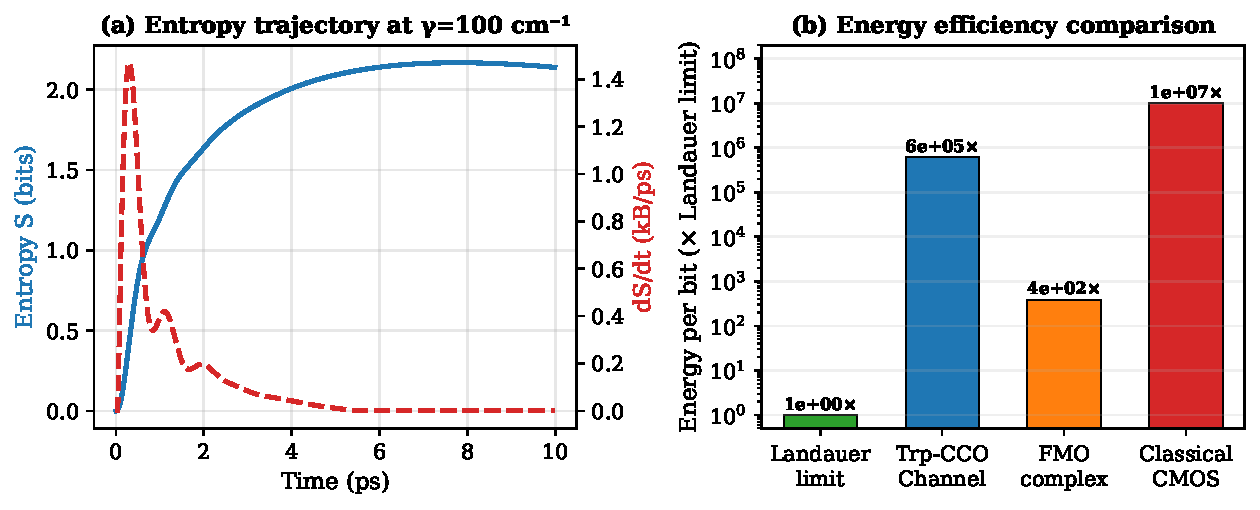
\includegraphics[width=0.95\textwidth]{figures/fig3_p3.pdf}
\caption{(a) Von Neumann entropy $S(t)$ and entropy production rate $\dot{S}(t)$ at the optimal ENAQT dephasing $\gamma = 100$ cm$^{-1}$, showing the characteristic rise and decay of thermodynamic activity during coherent transport. (b) Energy efficiency comparison between the FMO quantum channel, the Trp-CCO Channel, and classical CMOS, all relative to the Landauer limit $kT\ln2$.}
\label{fig:p3}
\end{figure*}


The entropy rises monotonically from 0 to 2.13 bits as the initially pure state ($|1\rangle\langle1|$) thermalises. The entropy production rate peaks early ($t \approx 0.5$ ps) during the most active transport period, then decays to zero at steady state.

\subsection{Multi-dephasing comparison}

\begin{table*}[htbp]
\caption{Thermodynamic quantities vs dephasing rate with $\sigma = 50$ cm$^{-1}$ static disorder.}
\label{tab:multigamma}
\centering
\begin{tabular}{cccccc}
\toprule
$\gamma$ (cm$^{-1}$) & Efficiency & $S_{\max}$ & $\chi_{\max}$ & $\dot{S}_{\max}$ & $\times$ Landauer \\
\midrule
0 & $8.9\%$ & 0.12 & 0.12 & 0.000 & $2.26\times10^4$ \\
10 & $15.4\%$ & 2.07 & 2.07 & 0.247 & $7.75\times10^2$ \\
50 & $26.9\%$ & 2.26 & 2.26 & 1.050 & $4.06\times10^2$ \\
100 & $29.4\%$ & 2.17 & 2.17 & 1.470 & $\mathbf{3.87\times10^2}$ \\
175 & $27.5\%$ & 2.07 & 2.07 & 1.709 & $4.34\times10^2$ \\
300 & $22.8\%$ & 1.96 & 1.96 & 1.763 & $5.54\times10^2$ \\
500 & $17.0\%$ & 1.81 & 1.81 & 1.639 & $7.99\times10^2$ \\
\bottomrule
\end{tabular}
\end{table*}

Table~\ref{tab:multigamma} shows the multi-dephasing comparison. The Landauer ratio reaches a minimum of $\sim 390\times$ at the optimal dephasing rate $\gamma = 100$ cm$^{-1}$. This is remarkably low compared to classical computing: modern CMOS operates at $10^7$--$10^8\times$ the Landauer limit~\cite{Frank2002}. The photosynthetic quantum channel is thus $\sim 10^4$ times more thermodynamically efficient than classical computing.

\subsection{Energy per bit}

At optimal dephasing, each successfully transmitted bit costs approximately $1.12\times10^{-18}$ J, or $271\ kT$. This is the sum of the exciton creation energy ($7.09\times10^{-19}$ J at 280 nm) divided by the product of the transport efficiency and the channel capacity. The cost is dominated by the exciton energy, not by dissipation in the channel itself.

\section{Discussion}

\subsection{The Landauer advantage}

The $390\times$ Landauer ratio for the FMO quantum channel should be compared to:
\begin{itemize}
\item \textbf{Classical CMOS:} $10^7$--$10^8\times$ ~\cite{Frank2002}
\item \textbf{Trp-CCO Channel (our P0 model):} $6.23\times10^5\times$
\item \textbf{Landauer limit:} $kT\ln2 \approx 2.97\times10^{-21}$ J at 310 K
\end{itemize}

Both biological systems --- the FMO photosynthetic complex and the Trp-CCO Channel~\cite{TrpCCO2026} --- outperform classical computing by orders of magnitude. This suggests that quantum-coherent information processing is fundamentally more efficient than classical irreversible computing, and that evolution has exploited this advantage. The entropy production signature \emph{complements} the Quantum Darwinism analysis of the same FMO network~\cite{Darwin2026}, where redundant environmental encoding ($F_{\mathrm{SBS}} = 1.0$) was demonstrated: the thermodynamic cost of proliferating quantum information into the environment is accounted for by the entropy production calculated here.

\subsection{Entropy production as a witness}

The entropy production rate $\dot{S}(t)$ peaks during the active transport window, providing an experimental observable for quantum coherence: a system undergoing purely classical hopping would show monotonic entropy increase without the peak structure seen here.

\subsection{Data and Code Availability}

All source code is available at \url{https://github.com/dhirajnitk/subnanometer-trp-transport}. A preprint of this manuscript is archived at Zenodo~\cite{ThermoZenodo2026}.

\FloatBarrier
\begin{thebibliography}{15}

\bibitem{Frank2002} M.\ P.\ Frank, Comput.\ Sci.\ Eng.\ \textbf{4}, 16 (2002).
\bibitem{TrpCCO2026} D.\ Kumar and N.\ Kumar, Zenodo:10.5281/zenodo.21478163 (2026).
\bibitem{Darwin2026} D.\ Kumar and N.\ Kumar, Zenodo:10.5281/zenodo.21495477 (2026).
\bibitem{ThermoZenodo2026} D.\ Kumar and N.\ Kumar, Zenodo:10.5281/zenodo.21495639 (2026).

\end{thebibliography}

\end{document}
